% ==================================================================
\section{问题一：多模态情感特征提取与时序对齐}\label{sec:q1}
% ==================================================================

问题一要求从附件1的原始视频出发，说清楚三件事：原始样本怎么处理，各模态的情感特征如何定义和提取，跨模态时序对齐按什么规则、怎样实现。三件事里真正难的是对齐。文本以“词”为单位，没有时间戳；语音按10毫秒一帧，一条几秒的片段就有几百帧；视觉按每秒10帧抽取。三者的时间尺度和时间轴都不一样，不统一到同一套序列位置上，下游模型就没法用。

本章先给出三路特征的提取方法，再给出三种对齐方案。三种方案共用同一个重采样算子，输出的形状完全一致，区别只在“时间轴怎么定义”：按词位置、按视频全程、按说话者可见的有效时段。第三种是本文提出的改进。

\subsection{原始样本与总体处理流程}\label{sec:q1flow}

附件1共100条英文视频，分布在37个以 video\_id 命名的子文件夹中，每个片段以 clip\_id.mp4 保存，时长在2.648～34.567秒之间，合计约777秒。标注表 label-100.xlsx 给出每条片段的转写文本 text、连续强度 label（$[-3,3]$）和极性 annotation。我们以“video\_id + clip\_id”作为样本编号，100条样本全部保留并逐条输出特征，没有替换、删除或修改任何样本和标签；若某条片段检测不到说话者的脸，按第\ref{sec:m3}节的退化规则处理，而不是把它剔除。

处理流程分两段。第一段是逐模态提取：文本经 BERT 编码成词元级向量，语音从视频中抽出后分帧提取声学描述子，视觉按固定帧率抽帧并做人脸检测后提取面部描述子。第二段是对齐：用三角核把三路长短不一的序列重采样到统一的50个序列位置，得到 text $(50,768)$、audio $(50,74)$、vision $(50,35)$ 三个矩阵，与附件2的 aligned\_50.pkl 形状一致。

\subsection{三模态情感特征的定义与提取}\label{sec:q1feat}

三路特征的定义见表\ref{tab:q1feat}。三路都使用开源工具或预训练模型，模型参数全部冻结，不做任何微调。

\begin{table}[htbp]
\centering
\caption{三模态情感特征的定义}
\label{tab:q1feat}
\begin{tabular}{>{\raggedright\arraybackslash}p{1.2cm}>{\raggedright\arraybackslash}p{2.7cm}>{\raggedright\arraybackslash}p{5.9cm}c>{\raggedright\arraybackslash}p{1.8cm}}
\toprule
模态 & 工具 / 模型 & 特征定义 & 维数 & 原始粒度 \\
\midrule
文本 & bert-base-uncased\cite{devlin2019bert} & WordPiece 分词，加 \texttt{[CLS]}、\texttt{[SEP]}，截断或补齐到50个词元，取最后一层 last\_hidden\_state & 768 & 词元 \\
语音 & ffmpeg + librosa\cite{mcfee2015librosa} & 16 kHz 单声道，25 ms 窗、10 ms 帧移；MFCC\cite{davis1980mfcc} 及其统计量、过零率、谱质心、谱带宽、谱滚降、色度、能量等声学描述子 & 74 & 10 ms 帧 \\
视觉 & OpenCV + YuNet\cite{wu2023yunet} & 10 fps 抽帧，取面积最大的人脸；人脸框的位置、尺寸、相对运动等几何量，加框内像素的亮度、对比度等统计量；无脸帧置零 & 35 & 0.1 s 帧 \\
\bottomrule
\end{tabular}
\end{table}

\textbf{文本。}BERT 的输出是上下文表示，同一个词在“not good”和“very good”里的向量不同，否定、程度这些对情感很关键的信息因此能保留下来。有效词元数 $L_{txt}$ 包含 \texttt{[CLS]} 和 \texttt{[SEP]}，100条样本平均为24.5，最长的样本恰好占满50个位置。

\textbf{语音。}MFCC 刻画音色，能量和过零率反映响度与清浊变化，谱质心、带宽、滚降反映声音的明暗与尖锐程度，色度则与音高有关。这些量合在一起，承载语气、语调、语速这类“怎么说”的情感线索。

\textbf{视觉。}YuNet 是一个轻量的人脸检测器，在 CPU 上逐帧运行也足够快。我们没有用表情识别模型，而是用人脸框的几何量和框内像素统计量描述头部姿态、运动幅度和面部可见性。这样做的好处是不依赖额外的表情标注，代价是对细微表情的刻画比较粗，这一点在第\ref{sec:eval}章的缺点里还会提到。

需要说明的是，74和35这两个维数是按赛题统一的输入接口选定的。附件2的语音、视觉特征来自 CMU-MOSEI 官方提取流程，语音部分为 COVAREP\cite{degottex2014covarep} 声学特征，与本文 librosa 特征的每一维含义并不相同。因此本章保证的是\textbf{形状和时序组织}与附件2一致，并不声称两套特征在数值上可以互换；问题二、三的模型也是在附件2自带的特征上训练的。

\subsection{跨模态时序对齐的规则与实现}\label{sec:q1align}

\subsubsection{公共算子：三角核重采样}

设某一模态的帧序列为 $\{(\tau_i,\mathbf{f}_i)\}$，$\tau_i$ 为第 $i$ 帧的时间戳，$\mathbf{f}_i$ 为特征向量。给定锚点时刻 $a$，用三角核加权平均得到该锚点上的特征：
\begin{equation}\label{eq:tri}
w_i(a)=\max\!\Big(0,\ 1-\frac{|a-\tau_i|}{b}\Big),\qquad
\hat{\mathbf{f}}(a)=\frac{\sum_i w_i(a)\,\mathbf{f}_i}{\sum_i w_i(a)},
\end{equation}
其中 $b$ 为核带宽，取相邻帧的间隔。离锚点越近的帧权重越大，超出带宽的帧权重为0，最后做归一化。这个算子把“不等长、不等帧率”的序列统一到任意给定的一组锚点上，三种对齐方案都用它，差别只在锚点放在哪里。

\subsubsection{方法一：按词位置对齐（口径H）}

以文本为锚，序列位置就是词元序号。文本天然是词元级的，直接占据第 $0$ 到第 $L_{txt}-1$ 行（第0行为 \texttt{[CLS]}，第 $L_{txt}-1$ 行为 \texttt{[SEP]}）。语音、视觉按“词在语音时段内均匀分布”的近似，把 $L_{txt}-2$ 个内容词对应到时间锚点上：
\begin{equation}\label{eq:anchorH}
a_t=\frac{t-1}{L_{txt}-3}\,D_{sp},\qquad
\mathbf{x}_m[t]=\begin{cases}\hat{\mathbf{f}}_m(a_t), & 1\le t\le L_{txt}-2,\\ \mathbf{0}, & \text{其他},\end{cases}\qquad m\in\{a,v\},
\end{equation}
其中 $D_{sp}$ 为语音时长，即 $\mathrm{linspace}(0,D_{sp},L_{txt}-2)$。\texttt{[CLS]}、\texttt{[SEP]} 和尾部补齐位置上的语音、视觉特征恒为零。

这样构造出来的零帧结构是：第0帧为零，有效长度 $L_a=L_{txt}-1$，其后全为零。这与第\ref{sec:align}节在附件2上实测到的 $L_a=\mathrm{nnz}(\texttt{input\_ids})-1$ 完全一致，也就是说口径H复刻了附件2的对齐方式。它的信息密度最高，每个位置都对应一个词；缺点是有效位置数随句子长短变化，而且“词匀速发音”只是近似。

\subsubsection{方法二：全程50等分}

抛开“词”这个锚，直接在视频全程 $[0,D]$ 上均匀放50个锚点：
\begin{equation}\label{eq:anchorT}
a_k=\frac{k}{49}\,D,\qquad k=0,1,\dots,49.
\end{equation}
语音、视觉按式(\ref{eq:tri})重采样到这50个锚点。文本没有时间戳，仍按均匀发音的近似把 $L_{txt}$ 个词元铺在 $[0,D]$ 上，第 $j$ 个词元的时刻取 $\tau_j=jD/(L_{txt}-1)$，再用同一个算子重采样。

这种做法最简单，三路都落在固定的50个时间位置上。问题在于片段开头结尾的静音、人转身或低头的时段，也被平均铺进了这50个位置，混入了与情感无关的内容。

\subsubsection{方法三：说话者人脸跟踪与有效时段50等分（本文改进）}\label{sec:m3}

一段视频里，人并不是从头到尾都在说话或做表情：开头结尾常有静音，中间可能转身、低头、走出画面。方法二把这些空白也塞进50个位置，既浪费位置，又稀释了有效信息。

那么该用什么判据划定“有效时段”？只看有没有声音（语音活动检测，VAD）不够，因为人不说话时仍然可能在做表情；只看画面里有没有人脸也不够，背景里的路人也会被检测到。我们最终采用的判据是：\textbf{说话者本人的脸在不在画面里}。三种典型情况的处理见表\ref{tab:m3rule}。

\begin{table}[htbp]
\centering
\caption{方法三的采集判据}
\label{tab:m3rule}
\begin{tabular}{lcc}
\toprule
情况 & 说话者的脸在画面中 & 是否采集 \\
\midrule
正在说话 & 在 & 是 \\
不说话但在做表情 & 在 & 是 \\
转身、低头或走出画面 & 不在 & 否 \\
\bottomrule
\end{tabular}
\end{table}

具体分三步实现。

\textbf{第一步，锁定说话者。}先用短时能量做 VAD：第 $j$ 帧的短时能量为 $e_j$，满足 $e_j\ge0.05\max_j e_j$ 的帧判为语音帧；短于0.15秒的语音段视为噪声剔除，短于0.25秒的静音间隙予以填补。在“正在说话且检测到人脸”的帧里取面积最大的人脸作为说话者，记其典型面积为 $A_s$。之所以取最大，是因为单人讲话的视频里说话者离镜头最近、脸最大，这样可以排除背景中的其他人。

\textbf{第二步，判定可见性。}对全片每一帧，只有检测到人脸且面积不小于 $\kappa A_s$ 时，才认为说话者可见：
\begin{equation}\label{eq:visible}
v(\tau)=\mathbb{1}\big[\,\text{检测到人脸}\ \wedge\ A(\tau)\ge\kappa A_s\,\big],\qquad \kappa=0.4,
\end{equation}
其中 $A(\tau)$ 为 $\tau$ 时刻最大人脸的面积。

\textbf{第三步，在有效时间轴上等分。}把所有可见时段首尾拼接，得到有效时间轴。形式上可以写成累积可见时长的映射
\begin{equation}\label{eq:effmap}
\varphi(\tau)=\int_0^{\tau}v(u)\,\mathrm{d}u,\qquad D_{eff}=\varphi(D),\qquad a_k=\frac{k}{49}\,D_{eff},\quad k=0,\dots,49.
\end{equation}
三路特征只保留落在可见时段内的帧（文本词元按均匀发音近似取时刻），时间戳经 $\varphi$ 映射到 $[0,D_{eff}]$ 后，再用式(\ref{eq:tri})重采样到50个锚点。

\textbf{退化保护。}如果某条片段全程都检测不到说话者的脸，即 $D_{eff}=0$，则退化为方法二的全程等分，保证不会输出全零特征。

图\ref{fig:q1scheme}用一条示意片段对比了三种方案的锚点位置。

\begin{figure}[htbp]
\centering
\begin{tikzpicture}[x=0.89cm, y=0.62cm,
  lab/.style={font=\small, anchor=east},
  sp/.style={fill=red!60, draw=none},
  fv/.style={fill=green!45!black!60, draw=none},
  anc/.style={draw=blue!70!black, line width=1.1pt}]
% 语音与可见性
\node[lab] at (-0.2,0.25) {语音活动};
\fill[sp] (1.0,0) rectangle (4.2,0.5); \fill[sp] (5.0,0) rectangle (9.5,0.5);
\node[lab] at (-0.2,-0.85) {说话者脸可见};
\fill[fv] (0.6,-1.1) rectangle (7.2,-0.6); \fill[fv] (8.0,-1.1) rectangle (11.4,-0.6);
\draw[dashed, gray] (7.2,0.8) -- (7.2,-8.6); \draw[dashed, gray] (8.0,0.8) -- (8.0,-8.6);
\node[font=\scriptsize, gray] at (7.6,1.2) {转头};
% 时间轴
\draw[-{Stealth[length=1.6mm]}] (0,-1.8) -- (12.4,-1.8) node[right, font=\small] {$\tau$};
\foreach \x/\l in {0/0, 12/D} {\draw (\x,-1.7) -- (\x,-1.9); \node[below, font=\small] at (\x,-1.9) {$\l$};}
% 方法一
\node[lab] at (-0.2,-3.4) {方法一};
\foreach \i in {0,...,11} {
  \pgfmathsetmacro{\c}{(\i==0 || \i==11) ? "black!15" : "blue!25"}
  \fill[\c] (\i*0.8+0.02,-3.75) rectangle (\i*0.8+0.78,-3.05);}
\foreach \i in {12,...,14} {\draw[black!30] (\i*0.8+0.02,-3.75) rectangle (\i*0.8+0.78,-3.05);}
\node[font=\scriptsize] at (0.4,-3.4) {CLS}; \node[font=\scriptsize] at (1.2,-3.4) {$w_1$}; \node[font=\scriptsize] at (2.0,-3.4) {$w_2$};
\node[font=\scriptsize] at (5.2,-3.4) {$\cdots$}; \node[font=\scriptsize] at (8.4,-3.4) {$w_{10}$}; \node[font=\scriptsize] at (9.2,-3.4) {SEP};
\node[font=\scriptsize, black!55] at (10.8,-3.4) {补零};
\node[font=\scriptsize, black!60, anchor=west] at (0,-4.45) {（横轴为词元序号，与时间无关）};
% 方法二
\node[lab] at (-0.2,-5.9) {方法二};
\foreach \x in {0.0,0.632,1.263,1.895,2.526,3.158,3.789,4.421,5.053,5.684,6.316,6.947,7.579,8.211,8.842,9.474,10.105,10.737,11.368,12.0}
  \draw[anc] (\x,-6.2) -- (\x,-5.6);
% 方法三
\node[lab] at (-0.2,-7.9) {方法三};
\fill[black!10] (0,-8.2) rectangle (0.6,-7.6); \fill[black!10] (7.2,-8.2) rectangle (8.0,-7.6); \fill[black!10] (11.4,-8.2) rectangle (12,-7.6);
\foreach \x in {0.6,1.126,1.653,2.179,2.705,3.232,3.758,4.284,4.811,5.337,5.863,6.389,6.916,8.242,8.768,9.295,9.821,10.347,10.874,11.4}
  \draw[anc] (\x,-8.2) -- (\x,-7.6);
\end{tikzpicture}
\caption{三种对齐方案的锚点示意。方法一按词位置，方法二在全程等分，方法三只在说话者可见的时段内等分（蓝色竖线为锚点，只画出20个，实际为50个；灰色为说话者不可见、被剔除的时段）}
\label{fig:q1scheme}
\end{figure}

从图\ref{fig:q1scheme}可以看出方法三的两个特点。第一，片段开头说话前的一小段，人没出声但脸在画面里，方法三照样采集，纯 VAD 会把它丢掉。第二，中间说话者转头的那一段，虽然还在出声，但脸不可见，方法三把它剔除了；这时视觉特征本来就缺失，剔除反而让保留下来的每个位置三路都是完整的。

\subsubsection{三种方案的对比}

三种方案的差异汇总在表\ref{tab:q1cmp}中。

\begin{table}[htbp]
\centering
\caption{三种对齐方案对比}
\label{tab:q1cmp}
\begin{tabularx}{\textwidth}{l*{3}{>{\centering\arraybackslash}X}}
\toprule
 & 方法一 & 方法二 & 方法三 \\
 & （口径H） & （全程50等分） & （说话者有效时段） \\
\midrule
时间轴 & 词元序号 & 视频全程 $[0,D]$ & 有效时段 $[0,D_{eff}]$ \\
有效位置数 & $L_{txt}-2$\newline（随句长变化） & 固定50 & 固定50 \\
剔除静音、无人时段 & 不涉及 & 否 & 是 \\
采集判据 & 无 & 无 & 说话者脸可见 \\
与附件2口径 & 一致 & 不同 & 不同 \\
输出形状 & \multicolumn{3}{c}{text $(50,768)$，audio $(50,74)$，vision $(50,35)$} \\
\bottomrule
\end{tabularx}
\end{table}

三种方案各有用处。方法一与附件2口径一致，适合需要与附件2接口对接的场合；方法二、三把位置固定为50个时间桶，便于做时间维度上的分析，其中方法三的信息密度更高。

\subsection{特征文件规范}\label{sec:q1file}

每条样本输出一个 NumPy 压缩文件（.npz），文件名为样本编号，三种方案分别存放在各自的结果目录中：
\begin{itemize}
\item 方法一：step1\_extract/results/q1\_features/
\item 方法二：step1\_time50/results/q1\_time50\_features/
\item 方法三：step1\_vad50/results/q1\_vad50\_features/
\end{itemize}
每个文件包含的字段见表\ref{tab:q1npz}，读取方式如下（sample\_id 为样本编号）：
\begin{lstlisting}[language=Python]
import numpy as np
f = "step1_vad50/results/q1_vad50_features/<sample_id>.npz"
d = np.load(f)
text = d["text"]         # (50, 768)
audio = d["audio"]       # (50, 74)
vision = d["vision"]     # (50, 35)
L_txt = int(d["L_txt"])  # tokens incl. [CLS]/[SEP]
\end{lstlisting}

\begin{table}[htbp]
\centering
\caption{特征文件字段}
\label{tab:q1npz}
\begin{tabularx}{\textwidth}{ll>{\raggedright\arraybackslash}X}
\toprule
字段 & 形状 & 含义 \\
\midrule
text & $(50,768)$ & 文本特征，BERT last\_hidden\_state \\
audio & $(50,74)$ & 对齐后的语音特征 \\
vision & $(50,35)$ & 对齐后的视觉特征 \\
text\_bert & — & BERT 的整数输入（词元编号等），用于回指原文 \\
L\_txt & 标量 & 有效词元数（含 \texttt{[CLS]}、\texttt{[SEP]}） \\
effective\_secs 等 & 标量 & 仅方法三：有效时长、说话段数 n\_segments、说话者脸可见帧数 face\_frames、语音帧数 voice\_frames、既有语音又见到脸的帧数 voice\_face\_frames \\
\bottomrule
\end{tabularx}
\end{table}

\textbf{时序组织的可核验性。}每个序列位置都能按规则还原到原始素材上。方法一中，第 $t$ 个位置对应第 $t$ 个词元，经 text\_bert 解码即得原文的词，对应的语音时刻为式(\ref{eq:anchorH})中的 $a_t$，视频帧号为 $\lfloor10a_t\rfloor$。方法二中，第 $k$ 个位置对应原视频的 $a_k$ 时刻。方法三中，第 $k$ 个位置对应有效时间轴上的 $a_k$，还原到原视频为 $\varphi^{-1}(a_k)$，可见时段由固定参数下的检测结果唯一确定，可以重算。填充规则统一为：有效位置之外全部补零，有效长度由 L\_txt（方法一）或非零位置（方法二、三）给出。

\subsection{全量结果汇总}\label{sec:q1res}

100条样本都输出了三种方案的特征文件。逐条的汇总表（样本编号、原始时长、有效词元数、有效时长、说话段数、各方案的非零位置数，以及统一的特征维度与对齐粒度）见附录\ref{app:q1}，整体统计见表\ref{tab:q1sum}。

\begin{table}[htbp]
\centering
\caption{附件1特征提取结果的整体统计（100条样本）}
\label{tab:q1sum}
\begin{tabular}{ll}
\toprule
项目 & 结果 \\
\midrule
样本数 & 100条，来自37个原始视频 \\
片段时长 & 2.648～34.567 s，合计约777 s \\
有效词元数 $L_{txt}$ & 平均24.5，最大50 \\
能量 VAD 判为说话的时长 & 约249 s，占总时长的32\% \\
方法三平均有效时长占比 $D_{eff}/D$ & 0.93 \\
方法三说话者脸可见帧占比 & 0.88 \\
特征维度 & text $(50,768)$，audio $(50,74)$，vision $(50,35)$ \\
对齐粒度 & 方法一为词级；方法二、三为50个时间桶 \\
\bottomrule
\end{tabular}
\end{table}

\subsection{对齐质量评估}\label{sec:q1eval}

附件1虽然带有情感标签，但只有100条，而且本章的语音、视觉特征与附件2不在同一个特征空间，没法直接拿问题二的模型去比较三种对齐的下游效果。因此我们从“每个位置能否被解释为原始素材的一段”这个角度评价对齐质量，用三个指标：
\begin{itemize}
\item \textbf{非零位置数} $N_m=\#\{t:\ \|\mathbf{x}_m[t]\|_2>10^{-8}\}$：50个位置里有多少真正有内容；
\item \textbf{有效时长占比} $D_{eff}/D$（方法三）：剔除空白后保留的时长比例；
\item \textbf{说话者脸可见帧占比}（方法三）：可见帧数与视觉总帧数之比，反映视觉采集的有效性。
\end{itemize}
100条样本的平均结果见表\ref{tab:q1eval}和图\ref{fig:q1nz}。

\begin{table}[htbp]
\centering
\caption{三种对齐方案的评估结果（100条平均）}
\label{tab:q1eval}
\begin{tabular}{lccc}
\toprule
指标 & 方法一 & 方法二 & 方法三 \\
\midrule
平均词元数 $L_{txt}$ & 24.5 & 24.5 & 24.5 \\
语音非零位置数（/50） & 22.5 & 50.0 & 48.0 \\
视觉非零位置数（/50） & 21.1 & 46.1 & 47.5 \\
有效时长占比 & — & — & 0.93 \\
说话者脸可见帧占比 & — & — & 0.88 \\
\bottomrule
\end{tabular}
\end{table}

\begin{figure}[htbp]
\centering
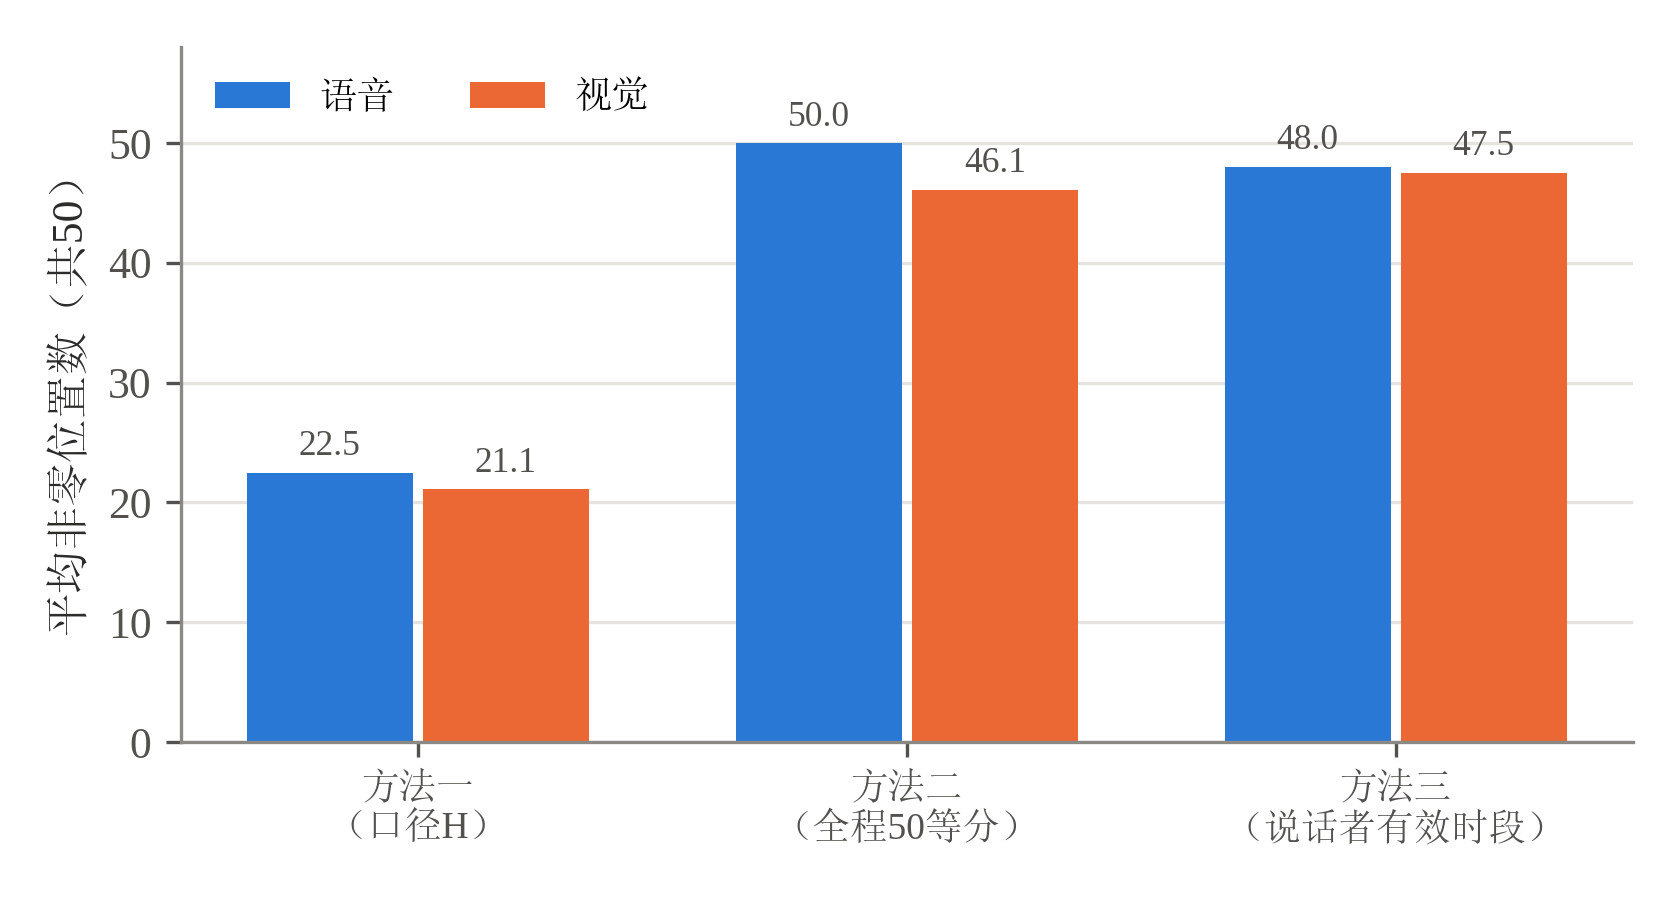
\includegraphics[width=0.72\textwidth]{figures/fig_q1_nonzero.png}
\caption{三种对齐方案下语音、视觉的平均非零位置数}
\label{fig:q1nz}
\end{figure}

方法一的语音非零位置为22.5，正好等于平均词元数减去 \texttt{[CLS]} 和 \texttt{[SEP]}（$24.5-2$），与式(\ref{eq:anchorH})的构造吻合：每个有内容的位置都对应一个词，最“干净”，信息密度最高。视觉只有21.1，比语音少1.4个，差额来自说话时恰好没检测到脸的那些词。

方法二的语音50个位置全部非零。这并不是好事：静音时段的声学特征也不是零，它被平均铺进了各个位置，混入了与情感无关的内容。

方法三剔除空白后，语音、视觉仍有48.0和47.5个非零位置，视觉还比方法二多了1.4个，说明它在保留几乎全部有效内容的同时，把位置让给了说话者可见的时段。

还有一组数字能说明为什么判据要选“说话者的脸”而不是“有没有声音”：按能量 VAD，100条片段总共777秒里只有约249秒在说话，占32\%。如果只按声音划定有效时段，三分之二的时长会被丢掉，其中包括大量不说话、但表情仍在变化的片段。按说话者脸可见来判定，平均只剪掉约7\%的时长；被剪掉的部分里，真正属于说话的只占全部语音帧的约8\%，而这些时刻视觉特征本来就缺失，剔除后反而保证了每个保留位置上三路特征都是完整的。

也要实事求是地说，在附件1上方法二和方法三的差别并不大。CMU-MOSEI 的片段大多是正对镜头的独白，说话者的脸88\%的时间都在画面里，可剔除的空白本来就少。方法三的优势在镜头切换多、人物频繁出画的视频上会更明显，这一点我们没有条件在本题数据上验证。

\subsection{典型样本验证}\label{sec:q1case}

我们选取了一条有代表性的样本：有效时长占比0.92，共30个词，含两段说话，样本编号为 \todo{样本编号}，文本为 \todo{文本片段}。图\ref{fig:q1case}最上方是音频能量包络，红色标出 VAD 判定的两段说话；下面三行依次是三种方案下 text、audio、vision 在50个位置上的非零填充模式。

\IfFileExists{figures/q1_typical_sample.png}{%
\begin{figure}[htbp]
\centering
\includegraphics[width=\textwidth]{figures/q1_typical_sample.png}
\caption{典型样本的音频能量与三种方案的特征填充模式}
\label{fig:q1case}
\end{figure}}{%
\begin{figure}[htbp]
\centering
\fbox{\parbox{0.9\textwidth}{\centering\vspace{1.5cm}\todo{把 eval/visualize\_sample.py 输出的图片重命名为 q1\_typical\_sample.png 放入 figures/ 后重新编译}\vspace{1.5cm}}}
\caption{典型样本的音频能量与三种方案的特征填充模式}
\label{fig:q1case}
\end{figure}}

从图中可以直接读出三种方案的差别：方法一只有词所在的位置非零，后面是整齐的补零；方法二把50个位置全部铺满，两段说话之间的静音也占了位置；方法三剔除了说话者不可见的时段，两段说话和其间仍在画面里的表情都得到保留。结合第\ref{sec:q1file}节的对应规则，任意一个位置都能还原到原文的词（方法一）或原视频的时刻与帧号（方法二、三），再回到视频中核对。

\subsection{可复现性说明}\label{sec:q1repro}

全部代码按方案分目录组织，每个目录内含 text\_feat.py、audio\_feat.py、vision\_feat.py、align.py 和入口 main.py，方法三另有 vad.py 与 face\_track.py；评估与可视化脚本在 eval 目录中。BERT 与 YuNet 的权重随代码包一并提供，无需另行下载。关键参数见表\ref{tab:q1param}，运行环境与命令见附录\ref{app:env}。

\begin{table}[htbp]
\centering
\caption{问题一的关键参数}
\label{tab:q1param}
\begin{tabularx}{\textwidth}{>{\raggedright\arraybackslash}p{4.4cm}>{\raggedright\arraybackslash}p{4.1cm}>{\raggedright\arraybackslash}X}
\toprule
参数 & 取值 & 说明 \\
\midrule
MAX\_POS & 50 & 统一的序列位置上限 \\
TEXT / AUDIO / VISION\_DIM & 768 / 74 / 35 & 三模态特征维度 \\
文本模型 & bert-base-uncased & 取最后一层隐状态，参数冻结 \\
音频 & 16 kHz，25 ms 窗 / 10 ms 帧移 & librosa 声学描述子 \\
视觉 & YuNet（2023mar 版 onnx），10 fps & 取面积最大的人脸 \\
对齐核 & 三角核 & 式(\ref{eq:tri}) \\
VAD\_ENERGY\_RATIO & 0.05 & 语音帧阈值为峰值短时能量的5\% \\
VAD\_MIN\_SPEECH / MAX\_GAP & 0.15 s / 0.25 s & 剔除短语音段 / 填补短静音 \\
FACE\_AREA\_RATIO（$\kappa$） & 0.4 & 说话者脸可见的面积比阈值 \\
SEED & 2026 & 随机种子 \\
\bottomrule
\end{tabularx}
\end{table}

\subsection{小结}

问题一用 BERT、librosa 和 YuNet 提取了768、74、35维的三路特征，并用同一个三角核算子给出了三种对齐方案。按词位置对齐的口径H与附件2的构造完全一致，每个位置对应一个词，可逐位回指原文；本文提出的说话者人脸跟踪方案，以“说话者的脸是否可见”划定有效时段，在100条样本上平均保留了93\%的时长，语音、视觉分别有48.0和47.5个非零位置，既剔除了无人时段，又没有丢掉不说话时的表情。
